\section{Grandezze e unità di misura}\label{sec:unità}
È necessario introdurre delle nuove grandezze fisiche per lo studio dei fenomeni astrofisici a causa degli ordini di grandezza elevati.
\subsection{Lunghezze}
Di seguito sono elencate le unità di misura maggiormente utilizzate per esprimere le lunghezze in astrofisica.
\begin{description}
    \item[Raggio solare] Non c'è bisogno di specificare a cosa si riferisce e vale $\si{\solarradius} \sim \SI{6.7e10}{cm}$. Nella tabella~\ref{tab:dimensioni-stelle} sono riportate le dimensioni di alcune stelle, per farsi un'idea degli ordini di grandezza. Si utilizza principalmente per la distanza di stelle e pianeti.
    \item[Unità astronomica] Esprime la distanza media tra Terra e Sole. Vale $\SI{1}{AU} \sim \SI{1.5e13}{cm}$. Si utilizza principalmente per indicare distanze riferite al sistema solare e dintorni.
    \item[Anno luce] Rappresenta la distanza che la luce percorre nel vuoto in un anno, si utilizza molto nei libri di divulgazione scientifica ma non in ricerca. Vale $\SI{1}{ly} \sim \SI{9.5e17}{cm}$. Nella tabella~\ref{tab:distanze-stelle} sono riportate le distanze di alcune stelle in anni luce.
    \item[parsec] Indica la distanza alla quale $\SI{1}{AU}$ sottende un angolo di $\ang{;;1}$ (\emph{secondo d'arco}), come mostrato in figura~\ref{fig:parsec}. Vale $\SI{1}{pc} = \SI{3.1e18}{cm}$. Nella tabella~\ref{tab:distanze-parsec} sono riportate le distanze di alcune strutture in parsec. Si utilizza principalmente in astrofisica galattica ed extra-galattica.
    \item[Redshift] Viene utilizzato per indicare distanze dell'universo lontano e in cosmologia.
\end{description}

\begin{table}
\caption{Dimensioni di alcune stelle}
\label{tab:dimensioni-stelle}
\centering
\begin{tabular}{ll}
\toprule
Stella & Dimensioni \\
\midrule
Stella più piccola          & $\sim \SI{0.084}{\solarradius}$ \\
Giove           & $\sim \SI{0.1}{\solarradius}$    \\
Super giganti rosse             & $\sim \SI{2000}{\solarradius}$  \\
Nane bianche & $\sim \SI{6000}{km}$  \\
Stelle di neutroni & $\sim \SI{10}{km}$  \\
\bottomrule
\end{tabular}
\end{table}

\begin{table}
\caption{Distanza di alcune stelle}
\label{tab:distanze-stelle}
\centering
\begin{tabular}{ll}
\toprule
Stella & Distanza da noi  \\
\midrule
Proxima Centauri & $\SI{4.2}{ly}$ \\
Sirio            & $\SI{8.6}{ly}$ \\
Betelgeuse       & $\SI{600}{ly}$ \\
\bottomrule
\end{tabular}
\end{table}

\begin{table}
\caption{Dimensioni di alcune strutture in parsec}
\label{tab:distanze-parsec}
\centering
\begin{tabular}{ll}
\toprule
Struttura & Dimensioni \\
\midrule
Galassie          & $\sim \textup{qualche} \, \si{kpc}$ \\
Via Lattea           & $\sim \SI{25}{kpc}$    \\
Ammassi di Galassie            & $\sim \textup{qualche} \, \si{Mpc}$  \\
Nubi di Magellano & $\sim \SI{60}{kpc}$  \\

\bottomrule
\end{tabular}
\end{table}

\begin{figure}
\centering
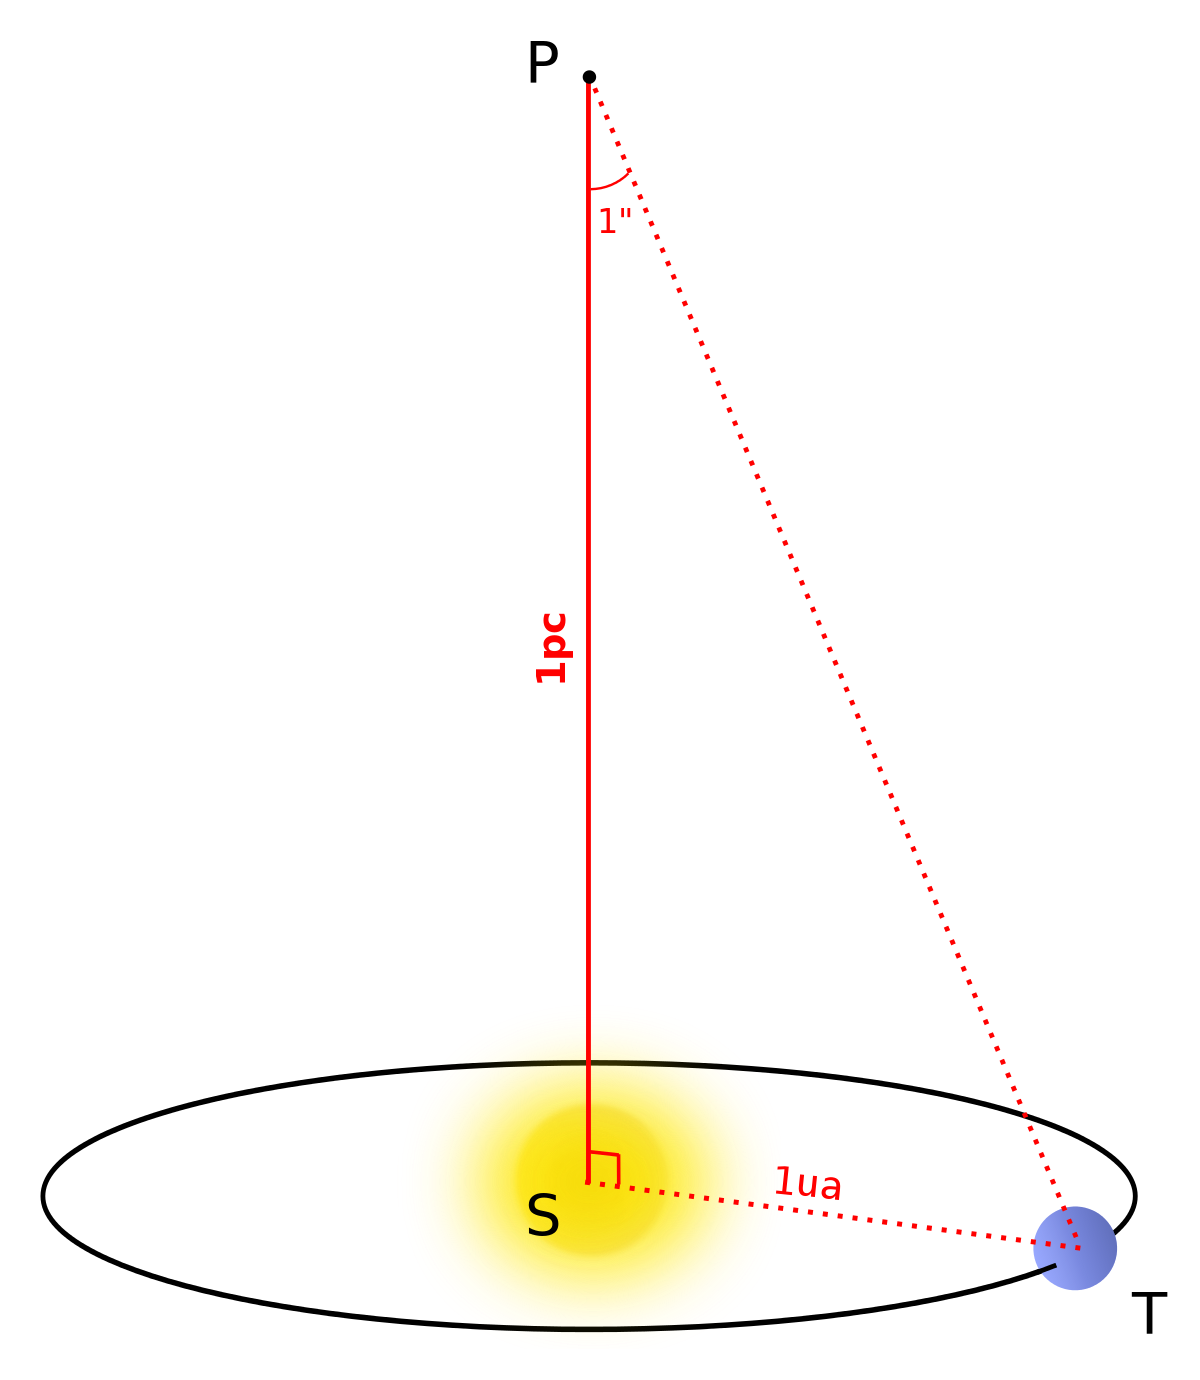
\includegraphics[width=0.5\textwidth]{immagini/parsec.png}
\caption{Definizione di parsec. $\SI{1}{pc}$ è la distanza alla quale $\SI{1}{AU}$ sottende un angolo di $\ang{;;1}$}
\label{fig:parsec}
\end{figure}

\subsection{Massa}
\begin{description}
    \item[Massa solare] Si spiega da sè. Vale $\si{\solarmass} = \SI{2e33}{g}$. In tabella~\ref{tab:masse-solari} sono presenti alcuni valori indicativi.
\end{description}

\begin{table}
\caption{Masse di alcune strutture}
\label{tab:masse-solari}
\centering
\begin{tabular}{ll}
\toprule
Struttura & Massa (\si{\solarmass}) \\
\midrule
Stelle          & $0.08$--$150$ \\
Ammassi stellari           & $10^3$--$10^6$    \\
Galassie            & $10^7$--$10^{13}$  \\
Ammassi di galassie & $10^{14}$--$10^{15}$  \\

\bottomrule
\end{tabular}
\end{table}

\subsection{Tempo}
Si utilizzano le solite unità di misura. In tabella~\ref{tab:età-strutture} sono riportati alcuni valori indicativi.
\begin{description}
    \item[Secondo]
    \item[Anno]
\end{description}

\begin{table}
\caption{Età di alcune strutture}
\label{tab:età-strutture}
\centering
\begin{tabular}{ll}
\toprule
Struttura & Età \\
\midrule
Stelle          & $\textup{qualche} \, \si{Myr}$--$\sim \SI{100}{Gyr}$ \\
Universo           & $t_H = \SI{13.7}{Gyr}$    \\


\bottomrule
\end{tabular}
\end{table}

\subsection{Posizione sulla sfera celeste}\label{sec:posizione-sfera-celeste}
Per \emph{sfera celeste} si intende una sfera di raggio unitario che dovrebbe essere centrata nell'osservatore, tuttavia, a seconda della convenienza, si considera in centro della sfera celeste coincidente con il \emph{centro della Terra} (sfera geocentrica), con il \emph{centro del Sole} (sfera eliocentrica) oppure con il \emph{baricentro del sistema solare} (sfera baricentrica). Se la distanza del corpo che si sta studiando è grande, scegliere uno dei tre diversi centri è del tutto equivalente. Si definisce \emph{equatore celeste} la proiezione dell'equatore terrestre sulla sfera celeste, si tratta di un cerchio massimo. Si definisce \emph{asse del mondo} la retta passante per il centro $O$ e perpendicolare al piano equatoriale. L'asse del piano definisce sulla sfera celeste due punti che prendono il nome di \emph{poli celesti}. Si faccia riferimento alla figura~\ref{fig:sfera-celeste}. Attualmente la croce del sud è vicina al polo sud terrestre, mentre il polo nord celeste è circa nella direzione della stella polare. A questo punto siamo pronti per introdurre l'\emph{eclittica}: è il cerchio massimo che descrive la traiettoria (apparente) del sole attorno alla Terra, in un anno. Ovvero, è l'intersezione tra la sfera celeste e il piano orbitale della Terra attorno al sole. Essa è inclinata di $\ang{23;27;}$ rispetto all'equatore celeste e interseca l'equatore in due punti opposti, detti \emph{equinozi}. Questi sono detti \emph{punto della Bilancia} e \emph{punto dell'Ariete}, quest'ultimo chiamato anche \emph{punto vernale} o \emph{equinozio di primavera}.

\begin{figure}
\centering
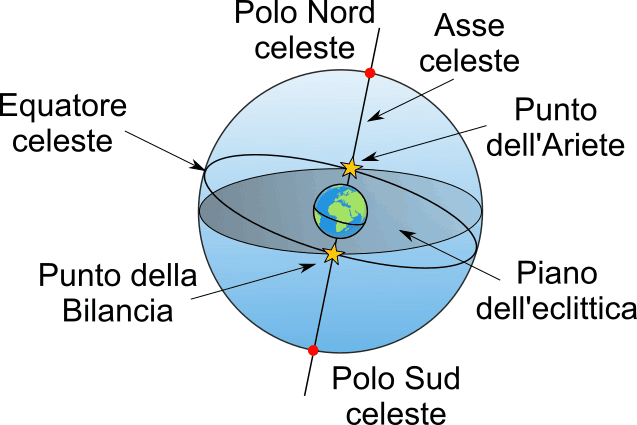
\includegraphics[width=0.5\textwidth]{immagini/sfera-celeste.png}
\caption{Sfera celeste. L'eclittica è l'intersezione tra la sfera celeste e il piano orbitale della Terra attorno al Sole. Essa interseca l'equatore terrestre in due punti opposti detti equinozi. Il punto dell'Ariete corrisponde all'equinozio di primavera (21 marzo), detto anche punto vernale.}
\label{fig:sfera-celeste}
\end{figure}

Lo \emph{Zenith} è il punto del cielo sopra la testa, ovvero la congiungente tra il centro della Terra e l'osservatore, cioè la verticale dell'osservatore. Si faccia riferimento alla figura~\ref{fig:zenith}. L'\emph{orizzonte astronomico} è il cerchio massimo formato dall'intersezione tra la sfera celeste e il piano perpendicolare alla verticale dell'osservatore. Ovviamente, l'osservatore è in grado di vedere solamente ciò che si trova sopra all'orizzonte astronomico. Si faccia attenzione al fatto che Zenith e orizzonte astronomico, dipendono dalla posizione dell'osservatore sulla Terra.

\begin{figure}
\centering
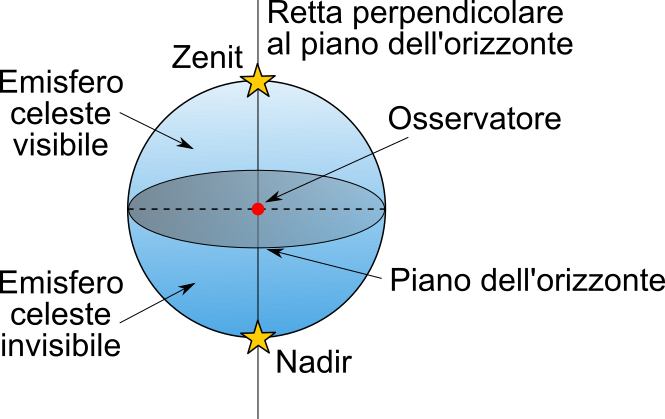
\includegraphics[width=0.5\textwidth]{immagini/zenit.png}
\caption{Zenith e orizzonte astronomico. L'osservatore vede solo ciò che sta sopra l'orizzonte astronomico. Dipendono da dove è posizionato l'osservatore sulla terra}
\label{fig:zenith}
\end{figure}

In ogni punto della Terra, la vedo ruotare attorno all'asse del mondo, che passa per i \emph{poli celesti}, di cui solamente uno è visibile sopra all'orizzonte (si vedi figura~\ref{fig:sfera-celeste}). Come vedo le stelle? Il loro moto avviene da est verso ovest ed è un moto rigido attorno all'asse del mondo. Quindi le distanze relative tra le stelle appaiono fisse, tuttavia ogni stella si muove di moto proprio, solo che le variazioni appaiono piccolissime a noi, che le osserviamo da lontano. Il periodo di rotazione delle stelle definisce il così detto \emph{giorno siderale}. Si faccia riferimento alla figura~\ref{fig:movimento-stelle} per capire come osserviamo il moto delle stelle.

\begin{figure}
\centering
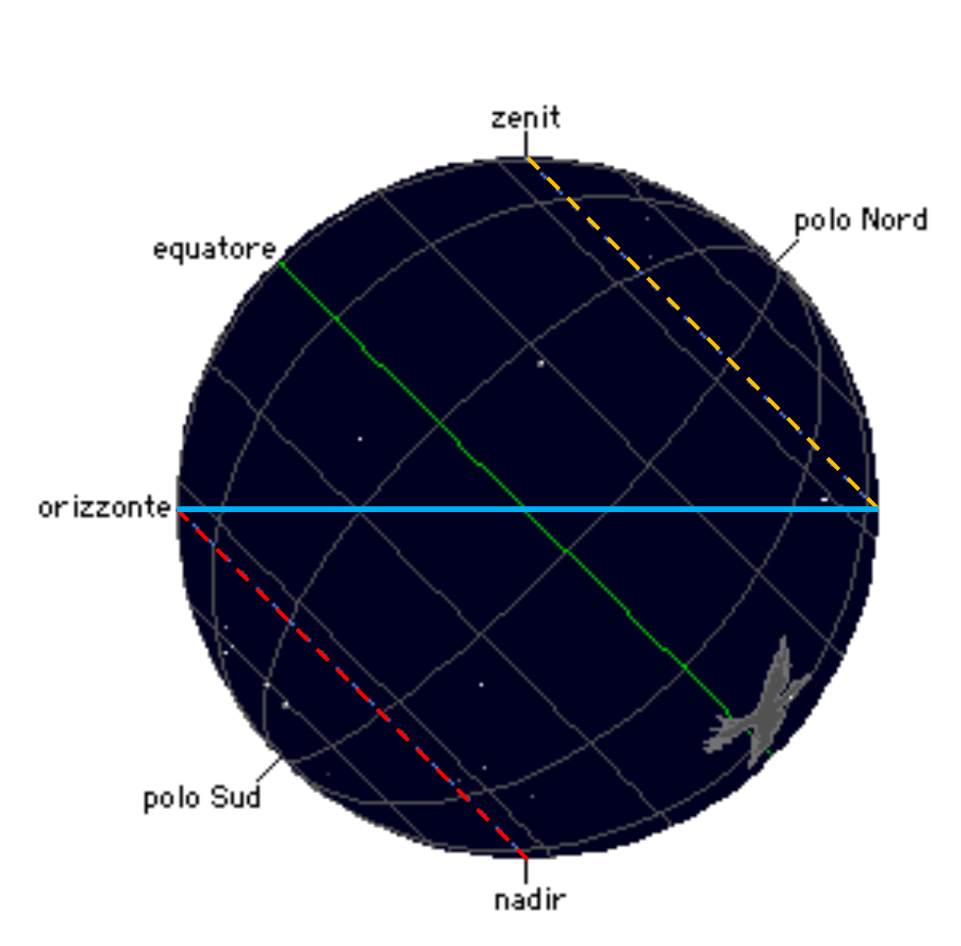
\includegraphics[width=0.5\textwidth]{immagini/movimento-stelle.png}
\caption{Come ci appare il movimento delle stelle. Tutte le stelle sopra il cerchio giallo non tramontano mai, quelle sotto il cerchio rosso non sorgono mai e le altre stelle le vediamo sorgere e tramontare}
\label{fig:movimento-stelle}
\end{figure}

Come definire un sistema di coordinate sulla sfera celeste? Si ricordi che noi osserviamo delle proiezioni su un piano, quindi sono sufficienti due coordinate. Conviene utilizzare delle coordinate angolari e il sistema di coordinate più utilizzato è il \emph{sistema equatoriale}. Esso usa come cerchi di riferimento l'equatore celeste e il meridiano\footnote{Un meridiano è un cerchio perpendicolare all'equatore.} passante per il punto vernale ($\gamma$). L'origine del sistema di coordinate è nel punto vernale, $O \equiv \gamma$, e ha per coordinate angolari l'ascensione della retta e la declinazione (figura~\ref{fig:sistema-equatoriale}).
\begin{description}
    \item[Ascensione retta (RA o $\alpha$)] distanza angolare tra il punto $\gamma$ e il meridiano dell'astro. Si misura in ore, minuti e secondi (hms), varia tra $0^h$ e $24^h$, aumentando verso E.
    \item[Declinazione (Dec o $\delta$)] distanza angolare tra l'equatore celeste e l'astro, lungo il meridiano dell'astro. Si misura in gradi, primi e secondi (gradi, arcominuti e arcosecondi), varia tra $\ang{0}$ e $+\ang{90}$ dall'equatore al polo N e tra $\ang{0}$ e $-\ang{90}$ dall'equatore al polo S.
\end{description}
Si faccia attenzione al fatto che i minuti e secondi d'orologio (RA) sono \emph{diversi} dai minuti e secondi d'arco (Dec). Utilizzando:
\[
    1^h = 60^m = 3600^s \qquad \ang{1} = 60' = 3600'' \qquad 24^h = \ang{360}
\]
si trova che:
\[
    1^h = \ang{15} \qquad 1^m = 15' \qquad 1^s = 15''
\]

\begin{figure}
\centering
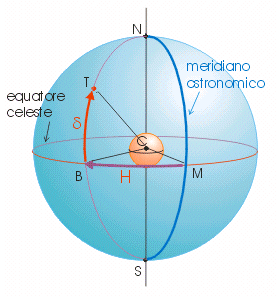
\includegraphics[width=0.5\textwidth]{immagini/sistema-equatoriale.png}
\caption{$\alpha$ è l'ascensione retta, ovvero la distanza angolare tra il punto $\gamma$ e il meridiano dell'astro, $\delta$ è la declinazione, ovvero la distanza angolare tra l'equatore celestre e l'astro, lungo il meridiano dell'astro.}
\label{fig:sistema-equatoriale}
\end{figure}

Si guardi la figura~\ref{fig:esempio-sistema-equatoriale} per un esempio sull'utilizzo di tale sistema di coordinate.

\begin{figure}
\centering
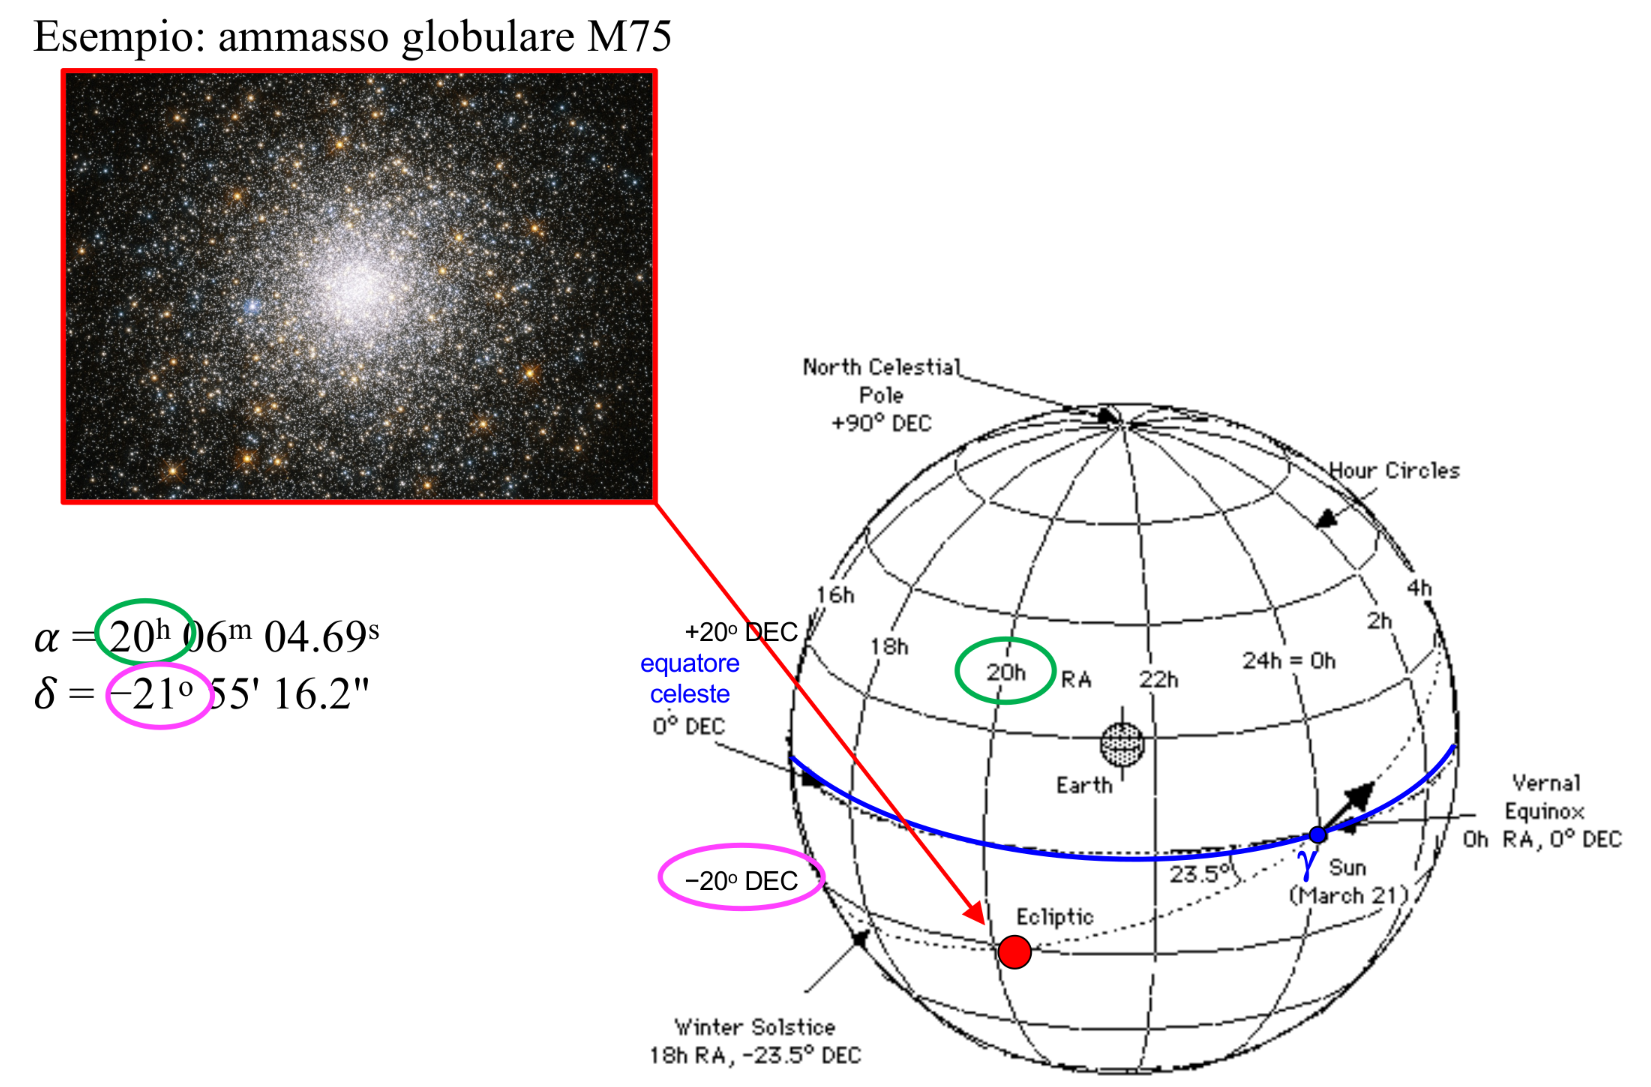
\includegraphics[width=\textwidth]{immagini/esempio-sistema-equatoriale.png}
\caption{Esempio di impiego delle coordinate del sistema equatoriale.}
\label{fig:esempio-sistema-equatoriale}
\end{figure}